\documentclass[letterpaper,11pt]{book}
\usepackage[toc,page]{appendix}
\usepackage{cergtheme}
\usepackage{afterpage}
\usepackage{amsmath,amssymb,latexsym,amsthm,amsfonts}
\usepackage[utf8]{inputenc}
\usepackage[table,svgnames,dvipsnames]{xcolor}%for coloring the cells and rows
%\usepackage{multirow}
\usepackage{fancyvrb}
\usepackage{verbatim}
\usepackage{tcolorbox}

\usepackage{graphicx,rotating}
\usepackage{enumerate}%enumerating with roman, alpha etc.
\usepackage{array,multirow}
\usepackage{multicol}
\usepackage{xcolor}
\usepackage{color}
%\usepackage[framed,numbered,autolinebreaks,useliterate]{mcode}%adding file as fgiures
%\usepackage{longtable}% for long tables spanning across multiple pages
%\usepackage{setspace}% for setting the line spacing
\usepackage{datetime}
%\onehalfspacing
\usepackage{amsmath}
\usepackage{algorithmic}
\usepackage{algorithm}
\usepackage{listings}
\usepackage{fullpage}%Using the full page
\usepackage{capt-of}%enables using caption without use of figure or table environment
\usepackage[pdftitle=FOBOS-CERG,pdfauthor=Panasayya Yalla,pdffitwindow=true, pdfcreator=Panasayya Yalla,
            pdfsubject=SideChannel\ Power Analysis\ ,pdfkeywords={Side Channel, Cryptography, Power Analysis, DPA},
            colorlinks=false]{hyperref}%For linking tables and figures in the document.

%\usepackage[usenames,dvipsnames]{xcolor}
%opening
\definecolor{cergpurple}{RGB}{64,5,116}
\definecolor{cergpink}{RGB}{128,35,145}
\definecolor{cerglightblue}{RGB}{140,159,229}
\definecolor{cergblue}{RGB}{100,116,172}

% box with mandatory title and options
\newtcolorbox{cergbox}[2][]{
   colframe=cergpurple,
   colback=cerglightblue!10!white,
   fonttitle=\bfseries,
   title = #2,
   #1
}

\renewcommand\familydefault{\rmdefault}
%%%%%setting for table boaders%%%%%
\setlength{\arrayrulewidth}{0.5mm}
\setlength{\tabcolsep}{18pt}
\renewcommand{\arraystretch}{1.0}% for streching the tables
%%%%%%%%%%%%%%%%%%%%%%%%%%%%%%%%%%%%%%%%%%%%%%%%%%
\usepackage{glossaries}
%\makeglossaries
\makeglossaries
%%%%%%%%%%%%%%%%%%%%%%%%%%%%%%%%%%%
% redefine \VerbatimInput
\RecustomVerbatimCommand{\VerbatimInput}{VerbatimInput}%
{fontsize=\footnotesize,
	%
	frame=lines,  % top and bottom rule only
	framesep=2em, % separation between frame and text
	rulecolor=\color{Gray},
	%
	%label=\fbox{\color{Black}data.txt},
	%labelposition=topline,
	%
	commandchars=\|\(\), % escape character and argument delimiters for
	% commands within the verbatim
	commentchar=*        % comment character
}





%%%%%%%%SETTING THE TITLE PAGE%%%%%%%%%%%%%%5
\usepackage{pdfcolmk}
%\pdftitle={Interface-CERG}
%\usepackage[svgnames]{xcolor}

%%%%%%%%%%%%%%%%%%Drawing folder structure
\usepackage{tikz}
\usetikzlibrary{trees}
%%%%%%%%%%%%%%%%%%%%%%%%%%%%%%%%%%%%%%%%%%%%%%%%%%%%%
%----------------------------------------------------------------------------------------
%   TITLE PAGE
%----------------------------------------------------------------------------------------
\newlength{\drop} % Command for generating a specific amount of whitespace
\newcommand*{\titleAT}
    {
    \begingroup % Create the command for including the title page in the document
    \centering % Center all text
    \drop=0.1\textheight % Define the command as 10% of the total text height
    \rule{\textwidth}{1pt}\par % Thick horizontal line
    \vspace{2pt}\vspace{-\baselineskip} % Whitespace between lines
    \rule{\textwidth}{0.4pt}\par % Thin horizontal line
    \vspace{0.25\drop} % Whitespace between the top lines and title
    
        \textcolor{black}
	{
            { \Huge \textbf{Flexible Opensource workBench }}\\
	    { \Huge \textbf{fOr}}\\
	    { \Huge \textbf{Side-channel analysis}}
    }    \\ 
        \drop=0.1\textheight % Define the command as 10% of the total text height
	\rule{\textwidth}{1pt}\par % Thick horizontal line
	\vspace{2pt}\vspace{-\baselineskip} % Whitespace between lines
	\rule{\textwidth}{0.4pt}\par % Thin horizontal line
	\vspace{0.25\drop} % Whitespace between the top lines and title
	{ \Large \textit{FOBOS User Guide $v1.0$}}\\
        %\title{FOBOS: A Prototype for Conducting Side-channel Evaluations on FPGAs}}\\[0.5\baselineskip] % Title line 1
        %\vspace{0.25\drop} % Whitespace between the title and short horizontal line
        %\rule{0.5\textwidth}{2.5pt}\par% Short horizontal line under the title
        %{\Huge{FOBOS Version 1.0}}\par
        \vspace{2.5\drop} % Whitespace between the thin horizontal line and the author name
        {\Large \textsc{Rajesh Velegalati, Panasayya Yalla \\ \& \\ Jens-Peter Kaps}}\\
        {\urlstyle{same}
		\nolinkurl{{rvelegal, pyalla, jkaps}'at'gmu.edu}} \par
            %{Email:\href{mailto:pyalla@gmu.edu}{pyalla@gmu.edu}}\par % Author name
        \vfill % Whitespace between the author name and publisher text
        %{\large \textcolor{Red}{\plogo}}\\[0.5\baselineskip] % Publisher logo
        {\large \textsc{George Mason University\\ Fairfax, Virginia}}\par % Publisher
                {\large \textit{ \today }}\par% Current date
        %{\large \textit{ October 15$^{th}$, 2015 }}\par% specific date
        %\vspace*{\drop} % Whitespace under the publisher text

        \begin{minipage}{\textwidth}
              \begin{minipage}[!t]{0.30\textwidth}
                \begin{center}
                     \vspace{1ex}
                    
\includegraphics[scale=0.35]{./themefigs/CERG-logo-sm.png}
                     % CERG-logo-sm.png: 200x150 pixel, 72dpi, 7.05x5.29 cm, bb=0 0 200 150
                \end{center}
            \end{minipage}
            \begin{minipage}[!t]{0.39\textwidth}
                 \hspace{3ex}
            \end{minipage}
            \begin{minipage}[!t]{0.30\textwidth}
		    \begin{center}    \begin{figure}
				    \centering
				    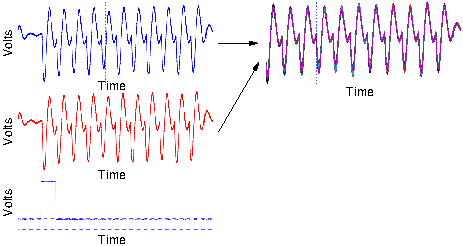
\includegraphics[scale=2.4]{../figures/tracealingment} 
			    \end{figure}
			
\includegraphics[scale=.50]{./themefigs/Mason-logo.png}
		\end{center}
            \end{minipage}
        \end{minipage}
        \rule{\textwidth}{0.4pt}\par % Thin horizontal line
        \vspace{2pt}\vspace{-\baselineskip} % Whitespace between lines
        \rule{\textwidth}{1pt}\par
        \begin{minipage}{\textwidth}
              \begin{minipage}[!t]{0.30\textwidth}
                \begin{center}
                     \vspace{1ex}
                    \href{https://cryptography.gmu.edu/}{www.cryptography.gmu.edu} % Thick horizontal line
                     % CERG-logo-sm.png: 200x150 pixel, 72dpi, 7.05x5.29 cm, bb=0 0 200 150
                \end{center}
            \end{minipage}
            \begin{minipage}[!t]{0.39\textwidth}
                 \hspace{3ex}
            \end{minipage}
            \begin{minipage}[!t]{0.30\textwidth}
		    \centering
                    \href{https://www.gmu.edu/}{www.gmu.edu} % Thick horizontal line
            \end{minipage}
        \end{minipage}
        %\href{http://cryptography.gmu.edu}{http://cryptography.gmu.edu} % Thick horizontal line
    \endgroup
    \clearpage
    \newcommand\blankpage{%
    \null
    \thispagestyle{empty}%
    \addtocounter{page}{-1}%
    \newpage}
    }
    
    
    \newcommand*{\titleATa}
        {
        \begingroup % Create the command for including the title page in the document
        \centering % Center all text
        \drop=0.1\textheight % Define the command as 10% of the total text height
        \rule{\textwidth}{1pt}\par % Thick horizontal line
        \vspace{2pt}\vspace{-\baselineskip} % Whitespace between lines
        \rule{\textwidth}{0.4pt}\par % Thin horizontal line
        \vspace{0.25\drop} % Whitespace between the top lines and title
        
            \textcolor{black}
    	{
                { \Huge \textbf{Flexible Opensource BOard }}\\
    	    { \Huge \textbf{for}}\\
    	    { \Huge \textbf{Side-channel analysis}}
        }    \\ 
            \drop=0.1\textheight % Define the command as 10% of the total text height
    	\rule{\textwidth}{1pt}\par % Thick horizontal line
    	\vspace{2pt}\vspace{-\baselineskip} % Whitespace between lines
    	\rule{\textwidth}{0.4pt}\par % Thin horizontal line
    	\vspace{0.25\drop} % Whitespace between the top lines and title
    	{ \Large \textit{FOBOS Reference Manual $v1.0$}}\\
            %\title{FOBOS: A Prototype for Conducting Side-channel Evaluations on FPGAs}}\\[0.5\baselineskip] % Title line 1
            %\vspace{0.25\drop} % Whitespace between the title and short horizontal line
            %\rule{0.5\textwidth}{2.5pt}\par% Short horizontal line under the title
            %{\Huge{FOBOS Version 1.0}}\par
            \vspace{\drop} % Whitespace between the thin horizontal line and the author name
            {\Large \textsc{Rajesh Velegalati, Panasayya Yalla \\ \& \\ Jens-Peter Kaps}}\\
            {\urlstyle{same}
    		\nolinkurl{{rvelegal, pyalla, jkaps}'at'gmu.edu}} \par
                %{Email:\href{mailto:pyalla@gmu.edu}{pyalla@gmu.edu}}\par % Author name
            \vfill % Whitespace between the author name and publisher text
            %{\large \textcolor{Red}{\plogo}}\\[0.5\baselineskip] % Publisher logo
            {\large \textsc{George Mason University\\ Fairfax, Virginia}}\par % Publisher
                    {\large \textit{ \today }}\par% Current date
            %{\large \textit{ October 15$^{th}$, 2015 }}\par% specific date
            %\vspace*{\drop} % Whitespace under the publisher text
    
            \begin{minipage}{\textwidth}
                  \begin{minipage}[!t]{0.30\textwidth}
                    \begin{center}
                         \vspace{1ex}
                        
\includegraphics[scale=0.35]{./themefigs/CERG-logo-sm.png}
                         % CERG-logo-sm.png: 200x150 pixel, 72dpi, 7.05x5.29 cm, bb=0 0 200 150
                    \end{center}
                \end{minipage}
                \begin{minipage}[!t]{0.39\textwidth}
                     \hspace{3ex}
                \end{minipage}
                \begin{minipage}[!t]{0.30\textwidth}
    		\begin{center}    
    			
\includegraphics[scale=.50]{./themefigs/Mason-logo.png}
    		\end{center}
                \end{minipage}
            \end{minipage}
            \rule{\textwidth}{0.4pt}\par % Thin horizontal line
            \vspace{2pt}\vspace{-\baselineskip} % Whitespace between lines
            \rule{\textwidth}{1pt}\par
            \begin{minipage}{\textwidth}
                  \begin{minipage}[!t]{0.30\textwidth}
                    \begin{center}
                         \vspace{1ex}
                        \href{https://cryptography.gmu.edu/}{www.cryptography.gmu.edu} % Thick horizontal line
			% CERG-logo-sm.png: 200\begin{figure}
			\centering
			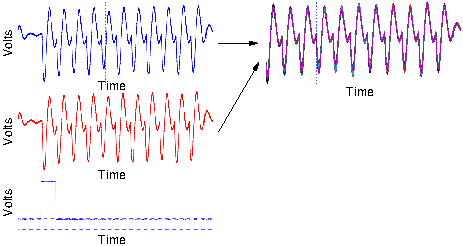
\includegraphics[scale=2.4]{../figures/tracealingment} 
		\end{figure}x150 pixel, 72dpi, 7.05x5.29 cm, bb=0 0 200 150
                    \end{center}
                \end{minipage}
                \begin{minipage}[!t]{0.39\textwidth}
                     \hspace{3ex}
                \end{minipage}
                \begin{minipage}[!t]{0.30\textwidth}
    		    \centering
                        \href{https://www.gmu.edu/}{www.gmu.edu} % Thick horizontal line
                \end{minipage}
            \end{minipage}
            %\href{http://cryptography.gmu.edu}{http://cryptography.gmu.edu} % Thick horizontal line
        \endgroup
        \clearpage
        \newcommand\blankpage{%
        \null
        \thispagestyle{empty}%
        \addtocounter{page}{-1}%
        \newpage}
        }
%\title{\Large{\textbf{Interface for Lightweight Implementations of \\Authenticated Cipher}}}
%\author{Panasayya Yalla \\ George Mason University}
%\date{}

%----------------------------------------------------------------------------------------
%   END OF TITLE PAGE
%----------------------------------------------------------------------------------------

%----------------------------------------------------------------------------------------
%   GLOSSARY 
%----------------------------------------------------------------------------------------

%----------------------------------------------------------------------------------------
%   END OF GLOSSARY
%------------------------------------------------------


%----------------------------------------------------------------------------------------
%   START OF DOCUMENT
%----------------------------------------------------------------------------------------


%----------------------------------------------------------------------------------------
%   Title Page
%----------------------------------------------------------------------------------------
\begin{document}
%%%%%%%%%%%%%%%%%%%%%%%%%%%%%%%%


%\pagenumbering{alph}
    %\maketitle
 { %\pagenumbering{gobble}
\thispagestyle{empty}
\titleAT % This command includes the title page
 \clearpage
 }
%%%%%%%%%%%%%%%%%%%%%%%%%%%%%%%%%%%%%%%%%%%%%%%%%%%%%%%%%%%%%%%%%%%%%%%%%%%%%%%%
{\pagenumbering{roman}
{\tableofcontents
%\clearpage
%\begin{appendix}
 \listoffigures
 \listoftables
 %%%%%%%%%%%%%%%%%%%%%%%%%%%%%55
 %PRINTING GLOSSARIES
 \newglossaryentry{SCA}
{
	name=SCA,
	description={Side Channel Attack}
}

\newglossaryentry{HD}
{
	name=HD,
	description={Hamming Distance}
}

\newglossaryentry{HW}
{
	name=HW,
	description={Hamming Weight}
}
 \printglossaries
 %%%%%%%%%%%%%%%%%%%%%%%%%%%%%%%5
  
%\end{appendix}
}}
\startofchapters
%\pagestyle{plain}
%\chapter{Side Channel Analysis}
\section{Introduction}% to Side-Channel Analysis}
Recent years have seen a dramatic increase of market adoption and utility of so called "smart" devices
by people from all walks of life. These devices play a central role in how people are entertained, communicate,
network, work, bank and shop. Yet for every positive outcome from these devices, there is often a corollary risk.
For example, let us consider a smart phone. On one hand, there are billions of applications which provide 
unprecedented ease of access to a plethora of applications or simply termed \emph{apps} to meet any user requirements. 
On the other hands, they are also are providing a fertile environment for the distribution of hostile apps or malware.
Also, the increased power of these smart phones makes them more suitable for a host of business purposes, which can also result
in the exposure and compromise of corporate data and systems. Finally, the very portability of mobile devices means that
they are highly susceptible to loss and theft. Thus there is great need in protecting information accessed by these devices
and this information is usually secured using cryptographic algorithms. 

According to Kerchoff's Law (or Shannon's Maxim)~\cite{klaws}, \newline
\parbox[c]{\textwidth}{\textit{a cryptosystem's security must be solely based on the 
		secret key even if everything about the underlying encryption algorithm is public knowledge.}} 
However, physical implementations in hardware as well as in software 
of such encryption algorithms have been shown to
leak secret information in the form of so called side-channels
and also during sudden change in operational characteristics of the crypto-device 
i.e. via \emph{Fault Injection}. The side-channel leakage could be in the 
form of power consumption~\cite{694}, electro magnetic radiation~\cite{811} or timing~\cite{694} 
of the device. The side-channels leak sensitive information whenever the device performs an 
operation using the secret data. Attacks which make use of such inhAnalysiserent physical leakage are called 
side-channel attacks \Gls{SCA}. \Gls{SCA} is a new research area of applied cryptanalysis that has
gained popularity since mid nineties. The research in this area shows that \Gls{SCA} pose a major 
threat because the physical implementations of the cryptographic
devices are difficult to control and often result in unintended leakage of information.
Generally, all hardware implementations of cryptographic algorithms are assumed to be vulnerable to side 
channel cryptanalysis, if there are no special precautions in the implementation.

\section{Power Analysis}
   \subsection{Simple Power Analysis (SPA)}
   \subsection{Differential/Correlation Power Analysis (DPA/CPA)}
       \subsubsection{Difference of Means}
        \subsubsection{Spearman Rank Coefficient}
        \subsubsection{Pearson's r}
      
   \subsection{Power Model}
%      \begin{itemize}
     \subsubsection{Hamming Distance (HD)}
     Hamming Distance \Gls{HD}
      \subsubsection{Hamming Weight (HW)}
      Hamming Weight \Gls{HW}
 %     \end{itemize}
/nhome/aabdulga/Documents/docs/UserGuide/fobos-overview.tex
\chapter{FOBOS Hardware Configuration} \label{chap:hardware-config}
\section{Introduction}
FOBOS consists of Python scripts for acquisition and analysis and hardware for controller and DUT.
This chapter describes the harware setup and descibes preparing and programming the controller and DUT boards.
This chapter assumes familiarity with Xilinx ISE and Xilinx Imapct tools.

FOBOS hardware is composed of two boards and other devices. The first board is the Control Board which handles communication with the control PC, triggering the oscilloscope and clocking the DUT.
The other board is the DUT which hosts the DUT Wrapper and the DUT.
An oscilloscope captures the power traces and the control PC collects them for analysis. 
A power supply is used to power the DUT and a clock generator might be used to provide clock for the Control Board which provides it to the DUT.

\begin{center}

\begin{figure}
  \label{fig:fobos-capture}
  \caption{FOBOS Hardware}
  \centering
   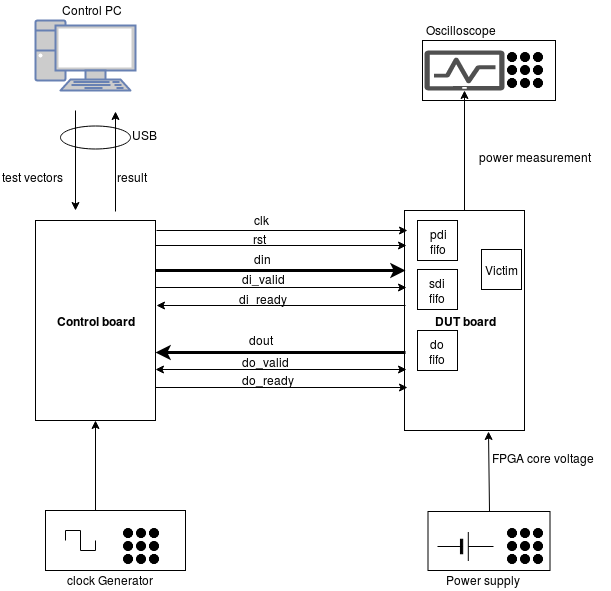
\includegraphics[scale=0.6]{../figures/FOBOS_Capture}
\end{figure}
\end{center}

\section{Hardware List}
\begin{enumerate}
  \item The control board (A standard FPGA board)
  \item The DUT board (A standard FPGA board)
  \item An oscilloscope (Agilent Technologies DSO6054A) 
  \item DC Power supply (Agilent E3620A)
  \item Clock generator (Instek SFG-2120 20 MHz)
  \item Control PC (A standard PC running Linux)
  \item Current probe (1mV/mA Tektronics CT-2 current sensing probe)
\end{enumerate}


\section{Programming the Control Board}

The source VHDL files for the controller are located at \texttt{fobos/source/vhdl}. You need to use Xilinx ISE to generate the bitstream file and use Xilinx Impact to load the bitstream
into the Control Board.

\subsection {Programming Steps}
\begin{enumerate}
  \item Create a new project using Xilinx ISE. In the New Project wizard, set the Project Settings per the control board used. 
  Make sure to select the values for Family, Device, Package and Speed (See Fig~\ref{fig:ctrl-design-properties} for an example).
  		\begin{figure} 
		\begin{center}
		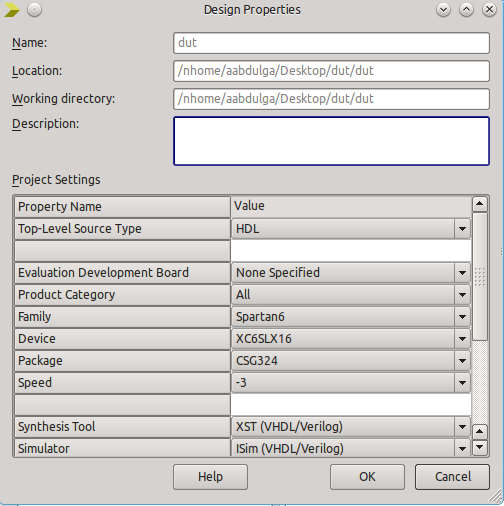
\includegraphics[scale=0.6]{figures/ctrl-design-properties}
		\caption{\label{fig:ctrl-design-properties}FOBOS Controller Desgin Properties}
		\end{center}
		\vspace{-1ex}
		\end{figure}
  \item From the Project menu, select Add Source... and add all files from \texttt{\$fobos/sources/common}.
  \item Repeat the previous step to add all vhdl files from \texttt{\$fobos/sources/vhdl/control}. Also, add the appropriate UCF file depending on the Control Board used (See Fig~\ref{fig:ctrl-add-sources}) .
		\begin{figure} 
		\begin{center}
		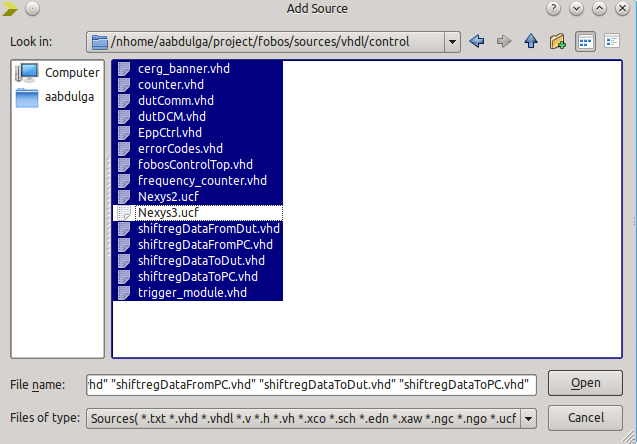
\includegraphics[scale=0.6]{figures/ctrl-add-sources}
		\caption{\label{fig:ctrl-add-sources}Adding Source Files to FOBOS Controller}
		\end{center} 
		\vspace{-1ex}
		\end{figure}
  \item Set the \texttt{fobosControlTopLevel} module as the top-level module for this project (See Fig~\ref{fig:ctrl-set-top-level}).
		\begin{figure} 
		\begin{center}
		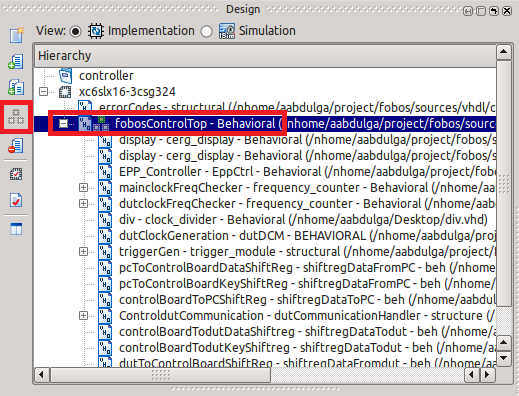
\includegraphics[scale=0.6]{figures/ctrl-set-top-level}
		\caption{\label{fig:ctrl-set-top-level}Setting Top-level Module}
		\end{center} 
		\vspace{-1ex}
		\end{figure}
  \item Generate the programming bit file for the control board by clicking "Generate Programming File" in the Processes window.
  \item Program the control board using Xilinx Impact. In the Processes window, click Configure Target Device (See Fig~\ref{fig:ctrl-run-impact}).
		\begin{figure} 
		\begin{center}
		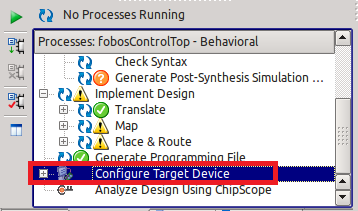
\includegraphics[scale=0.6]{figures/ctrl-run-impact}
		\caption{\label{fig:ctrl-run-impact}}
		\end{center}
		\vspace{-1ex}
		\end{figure}
  \item In the Impact window, click "Boundary Scan" then form the File menu, click "Initialize Chain" and assign the bit file to the FPGA. Now you may right-click the FPGA and click "Program".
		\begin{figure} 
		\begin{center}
		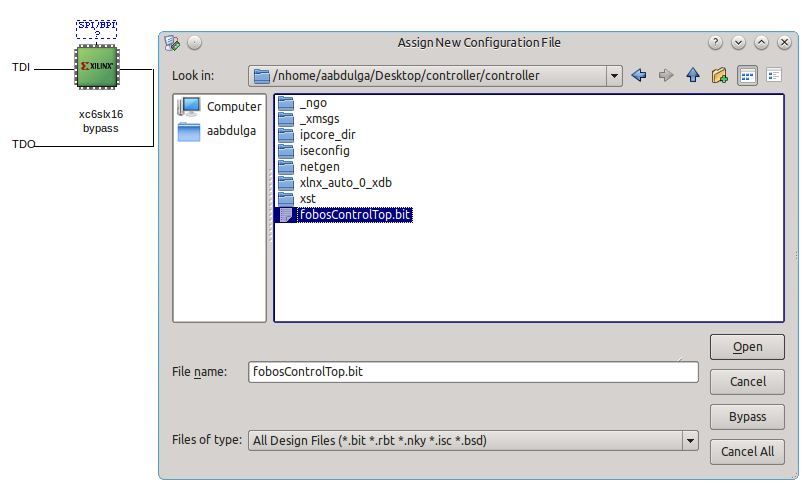
\includegraphics[scale=0.6]{figures/ctrl-program}
		\caption{\label{fig:ctrl-program}Progrmamming the Control Board}
		\end{center}
		\vspace{-1ex}
		\end{figure}
  \end{enumerate}

\section{DUT Board Programming}
The DUT board hosts two components:
\begin{enumerate}
 \item The DUT Wrapper : handles communication with the Control Board.
 \item The DUT (Victim) : the Device-Under-Test is user provided. This section assumes that this component is developed, instantiated and tested. Please see Chapter~\ref{chap:dut-dev} for more details.
\end{enumerate}

\subsection {Programming Steps}
\begin{enumerate}
  \item Create a new project using Xilinx ISE. In the New Project wizard set the Project Settings per the DUT Board used. 
  Make sure to select the values for Family, Device, Package and Speed (See Fig~\ref{fig:dut-design-properties} for an example).
		\begin{figure} 
		\begin{center}
		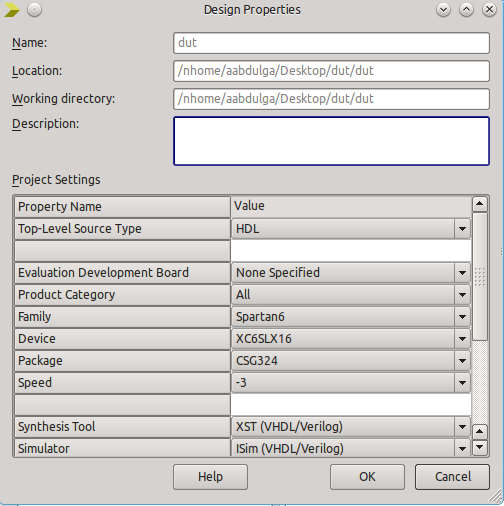
\includegraphics[scale=0.6]{figures/dut-design-properties}
		\caption{\label{fig:dut-design-properties}DUT Design Properties}
		\end{center}
		\vspace{-1ex}
		\end{figure}
  \item From the Project menu select Add Source... and add all files from \texttt{\$fobos/sources/common}.
  \item Repeat the previous process to add all vhdl files from \texttt{\$fobos/sources/vhdl/DUT} and make sure to add the appropriate UCF file depending on the DUT board used (See Fig~\ref{fig:dut-add-sources}).
  	\item Add the DUT (victim) vhdl files to the project (user provided).
		\begin{figure} 
		\begin{center}
		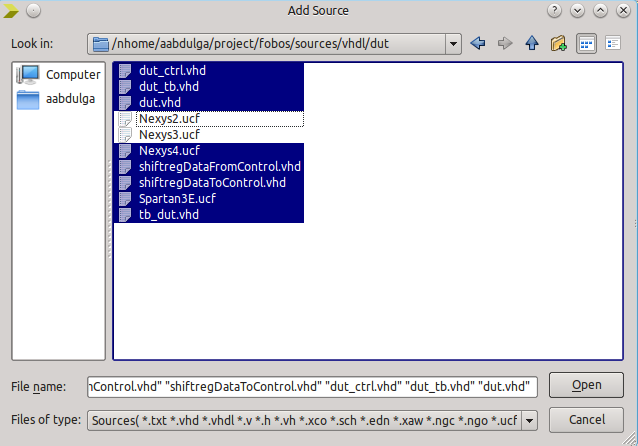
\includegraphics[scale=0.6]{figures/dut-add-sources}
		\caption{\label{fig:dut-add-sources}DUT Add Sources}
		\end{center}
		\vspace{-1ex}
		\end{figure}
  \item (Optional) You may choose to avoid using block RAMs in the implementation since this may affect attack difficulty.
     \begin{enumerate}
	\item Make sure to select the "Implementation" view.
        \item Right-click the Synthesize-XST process.
	\item In the Preocess Properties window, select HDL Options and select "Distributed" for the RAM Style property (See Fig~\ref{fig:dut-ram-style}).
	\item Click OK.
		\begin{figure} 
		\begin{center}
		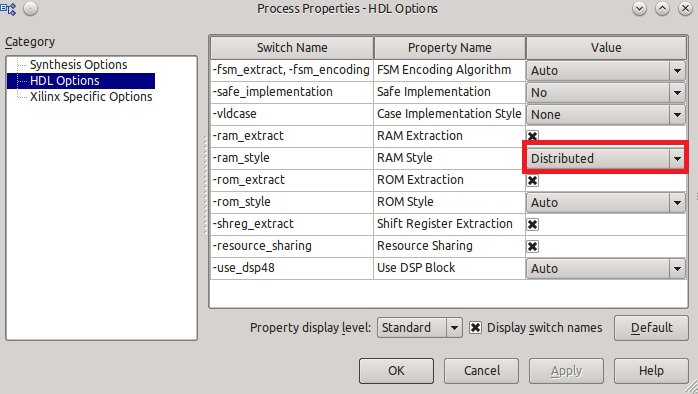
\includegraphics[scale=0.6]{figures/dut-ram-style}
		\caption{\label{fig:dut-ram-style}DUT RAM Style}
		\end{center}
		\vspace{-3ex}
		\end{figure}
     \end{enumerate}
  \item Set \texttt{FOBOS\_DUT} as the top-level module in this project.
		\begin{figure} 
		\begin{center}
		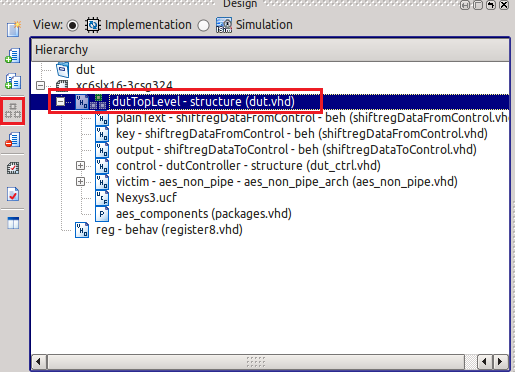
\includegraphics[scale=0.6]{figures/dut-set-top-level}
		\caption{\label{fig:dut-set-top-level}Set DUT Top-level}
		\end{center}
		\vspace{-3ex}
		\end{figure}
  \item Generate the programming bit file for the DUT by clicking "Generate Programming File" in the Processes window.
  \item Program the DUT using Xilinx Impact. In the Processes window, click Configure Target Device (See Fig~\ref{fig:dut-run-impact}).
		\begin{figure} 
		\begin{center}
		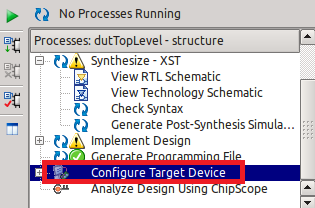
\includegraphics[scale=0.6]{figures/dut-run-impact}
		\caption{\label{fig:dut-run-impact}}
		\end{center}
		\vspace{-3ex}
		\end{figure}
  \item In the Impact window, click "Boundary Scan" then form the File menu, click "Initialize Chain" and assign the bit file to the FPGA. Now you may right-click the FPGA and click "Program".
		\begin{figure} 
		\begin{center}
		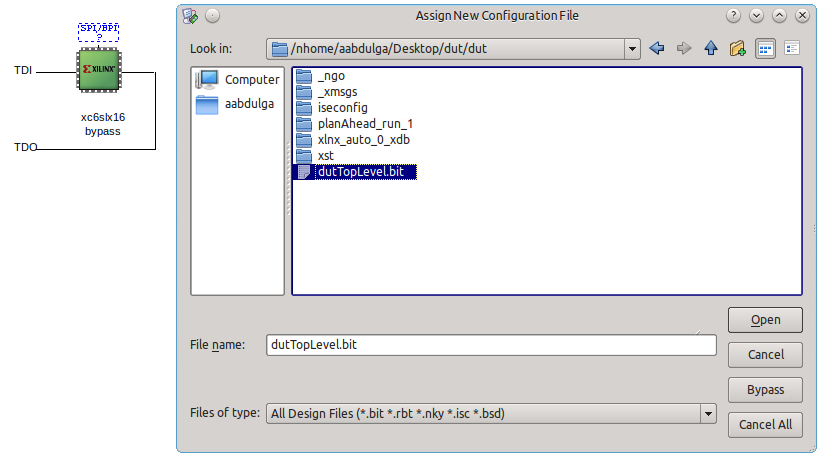
\includegraphics[scale=0.6]{figures/dut-program}
		\caption{\label{fig:dut-program}Progrmamming DUT}
		\end{center}
		\vspace{-3ex}
		\end{figure}
  \end{enumerate}


\section{Oscilloscope Configuration}
Ocsilloscope is connected to the PC via Ethernet. IP configuration must be completed on the oscilloscope for the PC to be able to collect traces. 
The oscillopscope used in current setup is Agilent DSO6054A. To configure IP on this oscilloscope, please refer to vendor's documentation.

\section{Connecting the Hardware}

To connect FOBOS hardware, follow these steps:
  \begin{enumerate}
  \item Connect control board to power and ground.
  \item Connect control board tirgger output the oscilloscope trigger channel.
  \item Connect the control board to the DUT (see details below).
  \item Connect the control board to the PC running FOBOS software using USB.
  \item Connect clock generator to control board. Set the clock generator to desired clock.
  \item Connect the current probe to the oscilloscope.
  \item Connect the current probe to the DUT's ground.
  \item Connect DUT to power making sure that the current probe is measuring the current.
  \item Connect DUT to power supply ground.
  \end{enumerate}
  
The following subsections ilustrate how to connect different FPGA boards as control and victim boards.

\subsection{Nexys3 Control Board - Nexys3 DUT}

This section describes connecting a Digilent Nexys3 Control board to a Nexys3 DUT board.
Nexys3 board includes a Xilinx Spartan6 FPGA. This board can use PMOD connectors for I/O.
It also descibes connections to other devices like the oscillopscope. For a high-level FOBOS hardware diagram, please refer to Figure~\ref{fig:fobos-capture}.

The two boards are connected using the PMOD port C and D. Some pins in port A and B are used to connect to the oscillopscope and the clock generator.
\newline
Note that the two boards must share GND. PMOD ports C and D are connected, each pin to its corresponding pin in the other board (e.g. JA1 $->$ JA1 and GND$->$ GND). 
However the 3.3 V pin is not connected in the PMOD connector.
\newline
\newline
\textbf{PMOD connector pin assignment on the control board}
\newline
\newline
\begin{array}{ | l | l | l | l | }
\hline
	PORT A & PORT B & PORT C & PORT D \\ \hline
	JA1: & JB1: EXTClock & JC1: DUTClock & JD1: reset \\ \hline
	JA2: & JB2: & JC2: do\_ready & JD2: di\_ready \\ \hline
	JA3: trigger  & JB3: & JC3: din(3) & JD3: dout(3) \\ \hline
	JA4: & JB4: & JC4: din(1) & JD4: dout(1) \\ \hline
	JA7: & JB7: & JC7: do\_valid & JD7: \\ \hline
	JA8: & JB8: & JC8: & JD8: di\_valid \\ \hline
	JA9: & JB9: & JC9: din(2) & JD9: dout(2) \\ \hline
	JA10: & JB10: & JC10: din(0) & JD10: dout(0) \\ \hline
\end{array}
\newline
\newline
\textbf{PMOD connector pin assignment on the DUT  board}
\newline
\newline
	\begin{array}{ | l | l | l | l | }
\hline
	PORT A & PORT B & PORT C & PORT D \\ \hline
	JA1: & JB1: & JC1: DUTClock & JD1: reset \\ \hline
	JA2: & JB2: & JC2: do\_ready & JD2: di\_ready \\ \hline
	JA3: & JB3: & JC3: din(3) & JD3: dout(3) \\ \hline
	JA4: & JB4: & JC4: din(1) & JD4: dout(1) \\ \hline
	JA7: & JB7: & JC7: do\_valid & JD7: \\ \hline
	JA8: & JB8: & JC8: & JD8: di\_valid \\ \hline
	JA9: & JB9: & JC9: din(2) & JD9: dout(2) \\ \hline
	JA10: & JB10: & JC10: din(0) & JD10: dout(0) \\ \hline
\end{array}


\newline

\chapter{Data Acquisition} \label{chap:dataAcquisition}

After test vectors have been generated, user can run dataAcquisition.py. The PC will send one test vector at a time to the control board, which sends it to DUT. 
The control board will trigger the oscilloscope to capture the power trace. The process will be repeated unitl all traces are collected.
 

The DUT Wrapper uses the header information in the test vector to put the data (plaintext, key etc.) into the correct FIFOs. 
The DUT Wrapper then allows the DUT (victim) algorithm to run by setting the victim reset to zero. The victim then drains the FIFOs (sdi,pdi and rdi FIFOs) and stores the output in the dout FIFO. 
Once the dout FIFO accumulates the expected amount of data, the DUT wrapper sends data to the controller which sends it to the PC.

Figure~\ref{fig:fobos-capture} shows the components of FOBOS including the handshake signals used.
Before running the \texttt{dataAcquisstion.py} script, the  user must  modify the configuration files at \texttt{config/config.txt} and \texttt{confi/acquisitionconfig.txt}.
Here is sample for \texttt{acquisitionConfig.txt} file.

\section{Data Aquisition Configuration}

\subsection{General Settings}
\begin{itemize}
 \item MEASUREMENT\_FORMAT \newline
 Possible values: dat \newline
 The format to store power measurements. Only dat is supported.
 \item LOGGING \newline 
 Possible values: INFO$|$DEBUG \newline
 The logging level. DEBUG is more verbose.
\end{itemize}

\subsection{Control Board Settings}
\begin{itemize}
 \item CONTROL\_BOARD \newline
 Possible values: Nexys3$|$Nexys2 \newline
 The Control Board type. 
 \item VICTIM\_RESET \newline
 Possible values: Integer \newline
 Reset the DUT after the specified clock cycles.
 \item TIME\_OUT \newline
 Possible values: Integer \newline
 If the DUT will not return data after the specified clock cycles, a time-out signal is returned to the PC.
\end{itemize}


\subsection{Trigger Settings}

The Control Board can send a trigger to the Oscilloscope once the DUT starts processing the data (ie. di\_ready = 0). Or it can be configured to trigger any number of clock cycles after this event occurs.
\begin{itemize}
 \item TRIGGER\_WAIT\_CYCLES \newline
 The number of clock cycles after which the trigger is asserted (after di\_ready goes to zero).
 \item TRIGGER\_LENGTH\_CYCLES \newline
 The time the trigger signal is asserted.
 \item TRIGGER\_TYPE \newline 
 possible values: TRG\_NORM, TRG\_FULL, TRG\_NORM\_CLK, TRG\_FULL\_CLK
        \begin{itemize}
          \item TRG\_NORM \newline Normal trigger mode. in this mode the TRIGGER\_WAIT\_CYCLES and TRIGGER\_LENGTH\_CYCLES are applied.
          \item TRG\_FULL \newline Full trigger mode. While DUT is running (between di\_ready = 0 and do\_valid = 1) the trigger is asserted.
          \item TRG\_NORM\_CLK \newline Similar to TRG\_NORM but the trigger signal is anded with the clock.
          \item TRG\_FULL\_CLK \newline Similar to TRG\_FULL but the trigger signal is anded with the clock.
       \end{itemize}

 \item CUT\_MODE \newline Controls how the trace retreived from the scope will be processed.
        possible values: FULL, TRIG\_HIGH
        \begin{itemize}
          \item FULL \newline The trace is cut starting at the rising edge of the trigger to the end of the screen.
          \item TRIG\_HIGH \newline the trace is cut from the rising edge to the falling edge of the trigger ie. the trace where the trigger is high will be saved.
        \end{itemize}
\end{itemize}  

\subsection{Data Settings}
\begin{itemize}
 \item DATA\_FILE \newline
 Possible values: file name (string) \newline
 The test-vector file name.
 \item EXPECTED\_OUTPUT \newline
 Possible values: Integer \newline
 Expected output size in bytes.
 \item OUTPUT\_FORMAT \newline
 Possible values: hex \newline
 Output format. 'hex' is the only supported format.
\end{itemize}

\subsection{Capture Settings}
\begin{itemize}
  \item NUMBER\_OF\_TRACES \newline
 Number of traces to collect.
 \item CAPTURE\_MODE  \newline
 Possible values: MULTI$|$SINGLE \newline
 Sigle encryption per traces or mutiple encryptions per trace.
\end{itemize}

\subsection{Oscilloscope Settings}
\begin{itemize}
 \item OSCILLOSCOPE \newline
 Possible values: AGILENT$|$OPENADC \newline
 Oscilloscope type.
 \item OSCILLOSCOPE\_IP \newline
 Possible values: IP address \newline
 Oscilloscope IP address.
 \item OSCILLOSCOPE\_PORT \newline
 Oscilloscope port number.
 \item AUTOSCALE = YES$|$NO \newline
 
 \item IMPEDANCE \newline
 Possible values: FIFTY$|$ONEMEG \newline
 Oscilloscope input impedance.
 \item CHANNELx\_RANGE  \newline
 Possible values: ON$|$OFF$|$voltage range \newline
 Oscilloscope channel voltage range (Full screen range) in Volts.
 \item TIME\_RANGE \newline
 Possible values: float (seconds)
 Oscilloscope time range in seconds (full screen time).
 \item TIMEBASE\_REF = LEFT    \newline
 \item TRIGGER\_THRESHOLD \newline
 Minimum voltage for valid trigger.
 \item TRIGGER\_SOURCE \newline
 Possible values: CHANNEL1$|$CHANNEL2$|$CHANNEL3$|$CHANNEL4 \newline
 Specifies the rigger channel.
 \item TRIGGER\_MODE =  EDGE
 \item TRIGGER\_SWEEP = NORM
 \item TRIGGER\_LEVEL = 1
 \item TRIGGER\_SLOPE = POSITIVE
 \item ACQUIRE\_TYPE = NORM$|$PEAK$|$HRES$|$AVER
 \item ACQUIRE\_MODE =  RTIM$|$ETIM$|$SEG

\end{itemize}

\section{Sample Configuration File}

\begin{verbatim}
 # ============================================= 
# Global Settings 
# ============================================= 
# ============================================= 
MEASUREMENT_FORMAT = dat # Default => dat 
LOGGING = INFO # INFO|DEBUG 
# ============================================= 
# ============================================= 
# Control Board Settings 
# ============================================= 
# ============================================= 
CONTROL_BOARD = Nexys3 
TRIGGER_WAIT_CYCLES = 0 #@VICTIM CLOCK 
TRIGGER_LENGTH_CYCLES = 1 #@VICTIM CLOCK 
TRIGGER_TYPE = TRG_FULL #TRG_NORM | TRG_FULL | TRG_NORM_CLK | TRG_FULL_CLK 
CUT_MODE = TRIG_HIGH #FULL | TRIG_HIGH 
# ============================================= 
# ============================================= 
# Test Data Generation Settings 
# ============================================= 
# ============================================= 
DATA_FILE     = dinFile.txt 
EXPECTED_OUTPUT = 16 # Expected output size in bytes 
OUTPUT_FORMAT = hex # Default => hex 
NUMBER_OF_ENCRYPTIONS_PER_TRACE = 1 
BLOCK_SIZE = 16 # In Bytes 
# ============================================= 
# ============================================= 
# FOBOS Capture Settings 
# ============================================= 
# ============================================= 
DUMMY_RUN = NO #YES/NO 
NUMBER_OF_TRACES = 50000 
#################################################### 
######## Signal Alignment Module Parameters ######## 
#################################################### 
CAPTURE_MODE = SINGLE # MULTI|SINGLE 
TRIGGER_THRESHOLD = 1.0 
# ============================================= 
# ============================================= 
# FOBOS Oscilloscope Settings 
# ============================================= 
# ============================================= 
# INTIALIZATION OPTIONS 
OSCILLOSCOPE = AGILENT #AGILENT|OPENADC 
OSCILLOSCOPE_IP = 192.168.10.10 
OSCILLOSCOPE_PORT = 5025 
AUTOSCALE = NO # YES|NO
IMPEDANCE = ONEMEG #FIFTY|ONEMEG 
# VOLTAGE AND TIME RANGE OPTIONS
CHANNEL1_RANGE = 0.060V 
CHANNEL2_RANGE = 6V 
CHANNEL3_RANGE = OFF # ON|OFF|voltage range 
CHANNEL4_RANGE = OFF # ON|OFF|voltage range 
TIME_RANGE = 0.000050 
TIMEBASE_REF = LEFT
# TRIGGER OPTIONS 
TRIGGER_SOURCE = CHANNEL2 
TRIGGER_MODE = EDGE
TRIGGER_SWEEP = NORM 
TRIGGER_LEVEL = 1 
TRIGGER_SLOPE = POSITIVE 
# ACQUIRE OPTIONS 
ACQUIRE_TYPE = NORM # NORM|PEAK|HRES|AVER 
ACQUIRE_MODE = RTIM # RTIM | ETIM| SEG
\end{verbatim}

\section{Running Data Acquisition}
Once the configuration is done, user can run 

\texttt{python dataAcquisition.py }

The output will be saved in \texttt{workspace/$<$projectName$>$/measurements}. The traces are stored in a Numpy array called \texttt{rawDataAligned.npy}.





\chapter{FOBOS Analysis}
\section{Power Model}
\section{Trace Alignment}
\section{Sample Window}
\section{Compression}
\section{Example}
\section{Files}
%\begin{figure}
%label=\fbox{\color{Black}data.txt},
%labelposition=topline,
%\VerbatimInput{./files/dataAnalysisParams.txt}
%\end{figure}
\begin{tcolorbox}[colback=yellow!10!white,colframe=green!75!black,title=dataAnalysisParams.txt]
	\textbf{Location:}fobos/bin/config/dataAnalysisParams.txt
	\tcblower
	\footnotesize
	\verbatiminput{./files/dataAnalysisParams.txt}
	\label{file:1}
\end{tcolorbox}
\begin{tcolorbox}[colback=yellow!10!white,colframe=green!75!black,title=compressionParams.txt]
	\textbf{Location:}fobos/bin/config/compressionParams.txt
	\tcblower
	\footnotesize
	\verbatiminput{./files/compressionParams.txt}
	\label{file:1}
\end{tcolorbox}
\begin{tcolorbox}[colback=yellow!10!white,colframe=green!75!black,title=postProcessesParams.txt]
	\textbf{Location:}fobos/bin/config/postProcessesParams.txt
	\tcblower
	\footnotesize
	\verbatiminput{./files/postProcessesParams.txt}
	\label{file:1}
\end{tcolorbox}
\begin{tcolorbox}[colback=yellow!10!white,colframe=green!75!black,title=projectPath.txt]
	\textbf{Location:}fobos/bin/config/projectPath.txt
	\tcblower
	\footnotesize
	\verbatiminput{./files/projectPath.txt}
	\label{file:1}
\end{tcolorbox}
\begin{tcolorbox}[colback=yellow!10!white,colframe=green!75!black,title=sampleSpaceDispParams.txt]
	\textbf{Location:}fobos/bin/config/sampleSpaceDispParams.txt
	\tcblower
	\footnotesize
	\verbatiminput{./files/sampleSpaceDispParams.txt}
	\label{file:1}
\end{tcolorbox}
\begin{tcolorbox}[colback=yellow!10!white,colframe=green!75!black,title=signalAlignmentParams.txt]
	\textbf{Location:}fobos/bin/config/signalAlignmentParams.txt
	\tcblower
	\footnotesize
	\verbatiminput{./files/signalAlignmentParams.txt}
	\label{file:1}
\end{tcolorbox}
\begin{tcolorbox}[colback=yellow!10!white,colframe=green!75!black,title=traceExpungeParams.txt]
	\textbf{Location:}fobos/bin/config/traceExpungeParams.txt
	\tcblower
	\footnotesize
	\verbatiminput{./files/traceExpungeParams.txt}
	\label{file:1}
\end{tcolorbox}

\begin{tcolorbox}[colback=yellow!10!white,colframe=green!75!black,title=config.txt]
	\textbf{Location:}fobos/bin/config/config.txt
	\tcblower
	\footnotesize
	\verbatiminput{./files/config.txt}
	\label{file:1}
\end{tcolorbox}

%\verbatiminput{./files/dataAnalysisParams.txt}
\chapter{Function Descriptions}

\section{FOBOS - Analysis Module}
FOBOS's analysis module uses a set of python scripts to post process the raw measurement data obtained from the oscilloscope and perform analysis on the obtained data.
Various functions implemented in the Analysis module is described below:\newline

\begin{table}
\caption{getAlignedMeasuredPowerData Function}
\begin{tabular}{ |p{2cm}||p{11cm}|  }
 \hline
 \multicolumn{2}{|c|}{\textbf{signalAnalysisModule.getAlignedMeasuredPowerData}} \\
 \hline
 Usage & \texttt{signalAnalysisModule.getAlignedMeasuredPowerData()}\\ \hline
 Inputs & None \\ \hline
 Outputs & M x N Numpy matrix that holds aligned traces. Where M is the number of traces and N is the number of samples per trace.\\ \hline
 Description & Reads aligned traces from the \$Workspace/\$projectName/\$attempt/Measurements directory and loads it to an M x N Numpy matrix.
This function calls signalAnalysisModule.readAlignedDataFromFile(). \\ \hline
\end{tabular}
\end{table}

\begin{table}
\caption{readAlignedDataFromFile Function}
\begin{tabular}{ |p{2cm}||p{11cm}|  }
 \hline
 \multicolumn{2}{|c|}{\textbf{signalAnalysisModule.readAlignedDataFromFile}} \\
 \hline
 Usage & \texttt{signalAnalysisModule.readAlignedDataFromFile()}\\ \hline
 Inputs & None \\ \hline
 Outputs & M x N Numpy matrix that holds aligned traces. Where M is the number of traces and N is number of samples per trace.\\ \hline
 Description & Reads aligned data from file and returns M x N Numpy matrix. \\ \hline
\end{tabular}
\end{table}

\begin{table}
\caption{detectSampleSize Function}
\begin{tabular}{ |p{2cm}||p{11cm}|  }
 \hline
 \multicolumn{2}{|c|}{\textbf{signalAnalysisModule.detectSampleSize}} \\
 \hline
 Usage & \texttt{signalAnalysisModule.detectSampleSize(fileName)}\\ \hline
 Inputs & Aligned traces file name. \\ \hline
 Outputs & Number of samples in a trace. \\ \hline
 Description & Reads the first 10 traces and returns the number of samples in the largest trace.
If the number of traces is less than 10 all traces are read.
This is done to be able to adjust all traces to the same number of samples if some do not have the same size due to acquisition timing. \\ \hline
\end{tabular}
\end{table}

\begin{table}
\caption{adjustSampleSize Function}
\begin{tabular}{ |p{2cm}||p{11cm}|  }
 \hline
 \multicolumn{2}{|c|}{\textbf{signalAnalysisModule.adjustSampleSize}} \\
 \hline
 Usage & \texttt{signalAnalysisModule.adjustSampleSize(sampleLength, dataArray)}\\ \hline
 Inputs & \begin{itemize} \item sample length to adjust to. 		   
         \item N x 1 nympy array that represents one trace where N is the number of samples in the trace. 
		\end{itemize}\\ \hline
 Outputs & SampleLenght x 1 Numpy array that represents the adjusted trace. \\ \hline
 Description & Used to modify the number of samples in a trace. If the number of samples is less than SampleLength, the array is padded with zeros. If the number of samples is more than SampleLength, the array is truncated. The function does nothing if the number of samples is equal to SampleLength.
 \\ \hline
\end{tabular}
\end{table}

\begin{table}
\caption{acquirePowerModel Function}
\begin{tabular}{ |p{2cm}||p{11cm}|  }
 \hline
 \multicolumn{2}{|c|}{\textbf{signalAnalysisModule.acquirePowerModel}} \\
 \hline
 Usage & \texttt{signalAnalysisModule.acquirePowerModel
 (HyptheticalDataFileName,globals.ADAPTIVE\_CPA)}\\ \hline
 Inputs & \begin{itemize}
 			\item Power model file name
 			\item  Correlation type 
 			\end{itemize}
 			\\ \hline
 Outputs & M x N Numpy array that holds the hypothetical power traces. Where N is the number of encryptions/decryptions and M is the number of key guesses. \\ \hline
 Description & Reads the hypothetical power data from file in \$fobos/data. Returns M x N Numpy array that holds the hypothetical power traces. Where N is the number of encryptions/decryptions and M is the number of key guesses.
 \\ \hline
\end{tabular}
\end{table}


\begin{table}
\caption{computeAlignedData Function}
\begin{tabular}{ |p{2cm}||p{11cm}|  }
 \hline
 \multicolumn{2}{|c|}{\textbf{signalAnalysisModule.computeAlignedData}} \\
 \hline
 Usage & \texttt{signalAnalysisModule.computeAlignedData(powerData, triggerData)}\\ \hline
 Inputs &  \begin{itemize}
 		    \item N x 1 Numpy array that holds measured power data. Where N is the number of samples.
 		    \item N x 1 Numpy array that holds trigger power data. Where N is the number of samples.
 		    \end{itemize} \\ \hline
 Outputs & Aligned power trace (K x 1 Numpy array where K is the number of samples). \\ \hline
 Description & Uses powerData and triggerData to generate the aligned trace.
The function looks for the rising edge of the trigger signal to determine the start of the trace. \\ \hline
\end{tabular}
\end{table}

\begin{table}
\caption{correlation\_pearson Function}
\begin{tabular}{ |p{2cm}||p{11cm}|  }
 \hline
 \multicolumn{2}{|c|}{\textbf{sca.correlation\_pearson}} \\
 \hline
 Usage & \texttt{sca.correlation\_pearson(measuredPowerData, hypotheticalPowerData)}\\ \hline
 Inputs &  \begin{itemize}
 		    \item M x N Numpy matrix for power traces. Where M is the number of encryptions/decryptions, N the number of samples per trace.
            \item L x M array the represents the hypothetical power values. Where M is the number of encryptions/decryptions and L is the number of key guesses (i.e for byte guess, L=256).
            \end{itemize}\\ \hline
 Outputs & N x L Numpy correlation matrix where N is the number of samples per trace. \\ \hline
 Description & Calculates Pearson correlation between the hypothetical data and measured data. Returns an N x L correlation matrix.
When we guess byte values L = 256.
 \\ \hline
\end{tabular}
\end{table}


\begin{table}
\caption{findMinimumGuessingEntropy Function}
\begin{tabular}{ |p{2cm}||p{11cm}|  }
 \hline
 \multicolumn{2}{|c|}{\textbf{sca.findMinimumGuessingEntropy}} \\
 \hline
 Usage & \texttt{signalAnalysisModule.computeAlignedData(measuredPowerData, triggerData)}\\ \hline
 Inputs &  \begin{itemize}
 		   \item measured power data.
 		   \item hypotheticalPowerData.
 		   \end{itemize}\\ \hline
 Outputs &  Minimum Guessing Entropy graph \\ \hline
 Description &  calculates the find Minimum Guessing Entropy \\ \hline
\end{tabular}
\end{table}



\begin{table}
\caption{plotTrace Function}
\begin{tabular}{ |p{2cm}||p{11cm}|  }
 \hline
 \multicolumn{2}{|c|}{\textbf{plottingModule.plotTrace}} \\
 \hline
 Usage & \texttt{plottingModule.plotTrace(dataToPlot, traceNos, plotType)}\\ \hline
 Inputs &  \begin{itemize}
 		   \item M x N Numpy matrix that holds traces to plot. Where M is the number of traces and N is the number of samples.
 		   \item Trace number
 		   \item Plot type
 		   \end{itemize}
per trace.
The traces to be plotted.
  \\ \hline
 Outputs & None \\ \hline
 Description & Plots the traces represented by the Numpy matrix. The x-axis represents time and the y-axis represents voltage. \\ \hline
\end{tabular}
\end{table}

\begin{table}
\caption{plotHist Function}
\begin{tabular}{ |p{2cm}||p{11cm}|  }
 \hline
 \multicolumn{2}{|c|}{\textbf{plottingModule.plotHist}} \\
 \hline
 Usage & \texttt{plottingModule.plotHist(corrMatrix, corrType)}\\ \hline
 Inputs &  \begin{itemize}
 		   \item M x N Correlation Numpy matrix. 
 		   \item Correlation type.
 		   \end{itemize}  \\ \hline
 Outputs & None \\ \hline
 Description & Plots a histogram. The x-axis represents the key guess and the y-axis represenst the number of occurrences.
 \\ \hline
\end{tabular}
\end{table}

\begin{table}
\caption{plotCorr Function}
\begin{tabular}{ |p{2cm}||p{11cm}|  }
 \hline
 \multicolumn{2}{|c|}{\textbf{plottingModule.plotCorr}} \\
 \hline
 Usage & \texttt{plottingModule.plotCorr(corrMatrix, corrType)}\\ \hline
 Inputs & \begin{itemize}
 		  \item M x N Numpy correlation matrix
 		  \item Correlation type 
 		  \end{itemize} \\ \hline
 Outputs & None \\ \hline
 Description & Plots correlation data. \\ \hline
\end{tabular}
\end{table}

\begin{table}
\caption{sampleSpaceDisp Function}
\begin{tabular}{ |p{2cm}||p{11cm}|  }
 \hline
 \multicolumn{2}{|c|}{\textbf{postProcessingModule.sampleSpaceDisp}} \\
 \hline
 Usage & \texttt{postProcessingModule.sampleSpaceDisp(alignedData)}\\ \hline
 Inputs & M x N Numpy matrix that holds aligned data. Where M is the number of traces and N is the number of samples per trace. \\ \hline
 Outputs & M x Window\_Size Numpy array that holds the aligned data after removing samples  \\ \hline
 Description & Removes samples before WINDOW\_START and after WINDOW\_START + WINDOW\_SIZE - 1 from each trace. \\ \hline
\end{tabular}
\end{table}

\begin{table}
\caption{compressData Function}
\begin{tabular}{ |p{2cm}||p{11cm}|  }
 \hline
 \multicolumn{2}{|c|}{\textbf{compressData}} \\
 \hline
 Usage & \texttt{compressData(measuredPowerData)}\\ \hline
 Inputs & M x N Numpy array that represents traces. Where M is the number of traces and N is the number of samples per trace. \\ \hline
 Outputs & M x K Numpy array that represents compressed traces. Where M is the number of traces and $K = \frac{N}{COMPRESSION\_LENGTH}$.  \\ \hline
 Description & Summarizes COMPRESSION\_LENGTH samples into one sample. The summarization type depends on the COMPRESSION\_TYPE configuration parameter which can be MEAN, MIN or Max. \\ \hline
\end{tabular}
\end{table}
\begin{table}
\caption{compress Function}
\begin{tabular}{ |p{2cm}||p{11cm}|  }
 \hline
 \multicolumn{2}{|c|}{\textbf{postProcessingModule.compress}} \\
 \hline
 Usage & \texttt{postProcessingModule.compress (a, compressionLenght, compressionType)}\\ \hline
 Inputs & \begin{itemize}
 		  \item M x N Numpy array that represents traces. Where M is the number of traces and N is the number of samples per trace.
 		  \item Number of samples to compress into one sample.
          \item Compression type.
          \end{itemize} \\ \hline
 Outputs &  M x K Numpy array that represents compressed traces. Where M is the number of traces and $K = \frac{N}{COMPRESSION\_LENGTH}$.  \\ \hline
 Description & This function is called by postProcessingModule.compressData() to do the compression. \\ \hline
\end{tabular}
\end{table}

\begin{table}
\caption{traceExpunge Function}
\begin{tabular}{ |p{2cm}||p{11cm}|  }
 \hline
 \multicolumn{2}{|c|}{\textbf{postProcessingModule.traceExpunge}} \\
 \hline
 Usage & \texttt{postProcessingModule.traceExpunge(measuredPowerData)}\\ \hline
 Inputs & M x N Numpy array that represents traces. Where M is the number of traces and N is the number of samples per trace. \\ \hline
 Outputs & L x N Numpy array that represents traces after removing the traces that do not fall in acceptable range. Where L is the number of traces and N is the number of samples per trace.  \\ \hline
 Description & Removes traces that do not fall in acceptable range. \\ \hline
\end{tabular}
\end{table}


\section{FOBOS - Capture Module}

The Capture module is used to run encryptions on hardware and capture traces from the ocsilloscope.

\begin{table}
\caption{openOscilloscopeConnection Function}
\begin{tabular}{ |p{2cm}||p{11cm}|  }
 \hline
 \multicolumn{2}{|c|}{\textbf{Oscilloscope\_core.openOscilloscopeConnection}} \\
 \hline
 Usage & \texttt{Oscilloscope\_core.openOscilloscopeConnection()}\\ \hline
 Inputs & None  \\ \hline
 Outputs &  None \\ \hline
 Description & Connects to oscilloscope. It opens a socket using the IP address OSCILLOSCOPE\_IP and port number OSCILLOSCPOE\_PORT. Also gets the oscilloscope identifier. \\ \hline
\end{tabular}
\end{table}

\begin{table}
\caption{setOscilloscopeConfigAttributes Function}
\begin{tabular}{ |p{2cm}||p{11cm}|  }
 \hline
 \multicolumn{2}{|c|}{\textbf{Oscilloscope\_core.setOscilloscopeConfigAttributes}} \\
 \hline
 Usage & \texttt{Oscilloscope\_core.setOscilloscopeConfigAttributes()}\\ \hline
 Inputs & None  \\ \hline
 Outputs &  None \\ \hline
 Description & Configures the oscilloscope by sending commands (in text format) to the oscilloscope. \\ \hline
\end{tabular}
\end{table}

\begin{table}
\caption{initializeOscilloscopeDataStorage Function}
\begin{tabular}{ |p{2cm}||p{11cm}|  }
 \hline
 \multicolumn{2}{|c|}{\textbf{Oscilloscope\_core.initializeOscilloscopeDataStorage}} \\
 \hline
 Usage & \texttt{Oscilloscope\_core.initializeOscilloscopeDataStorage()}\\ \hline
 Inputs & None \\ \hline
 Outputs &  None \\ \hline
 Description & Creates empty Numpy arrays for each enabled oscilloscope channel. \\ \hline
\end{tabular}
\end{table}

\begin{table}
\caption{armOscilloscope Function}
\begin{tabular}{ |p{2cm}||p{11cm}|  }
 \hline
 \multicolumn{2}{|c|}{\textbf{Oscilloscope\_core armOscilloscope}} \\
 \hline
 Usage & \texttt{Oscilloscope\_core.armOscilloscope()}\\ \hline
 Inputs & None \\ \hline
 Outputs &  None \\ \hline
 Description & Instructs the oscilloscope to digitize channels specified in FOBOS configuration. \\ \hline
\end{tabular}
\end{table}

\begin{table}
\caption{populateOscilloscopeDataStorageAndAlign Function}
\begin{tabular}{ |p{2cm}||p{11cm}|  }
 \hline
 \multicolumn{2}{|c|}{\textbf{Oscilloscope\_core.populateOscilloscopeDataStorageAndAlign}} \\
 \hline
 Usage & \texttt{Oscilloscope\_core.populateOscilloscopeDataStorageAndAlign(traceCount)}\\ \hline
 Inputs & The number of current trace. \\ \hline
 Outputs &  None \\ \hline
 Description & Reads power data trace from oscilloscope and trigger signal trace. It then aligns the trace to the trigger signal and saves the aligned trace to file. \\ \hline
\end{tabular}
\end{table}


\begin{table}
\caption{closeOscilloscopeConnection Function}
\begin{tabular}{ |p{2cm}||p{11cm}|  }
 \hline
 \multicolumn{2}{|c|}{\textbf{Oscilloscope\_core.closeOscilloscopeConnection}} \\
 \hline
 Usage & \texttt{Oscilloscope\_core.closeOscilloscopeConnection()}\\ \hline
 Inputs & None \\ \hline
 Outputs &  None \\ \hline
 Description & Closes socket that connects to oscilloscope. \\ \hline
\end{tabular}
\end{table}

\begin{table}
\caption{openControlBoardConnection Function}
\begin{tabular}{ |p{2cm}||p{11cm}|  }
 \hline
 \multicolumn{2}{|c|}{\textbf{Oscilloscope\_core.openControlBoardConnection}} \\
 \hline
 Usage & \texttt{usbcomm\_core.openControlBoardConnection()}\\ \hline
 Inputs & None \\ \hline
 Outputs &  None \\ \hline
 Description & Initializes connection to control board, resets control board and reads control board and victim clocks. \\ \hline
\end{tabular}
\end{table}

\begin{table}
\caption{initializeControlBoardConnection Function}
\begin{tabular}{ |p{2cm}||p{11cm}|  }
 \hline
 \multicolumn{2}{|c|}{\textbf{usbcomm\_core.initializeControlBoardConnection}} \\
 \hline
 Usage & \texttt{usbcomm\_core.initializeControlBoardConnection()}\\ \hline
 Inputs & None \\ \hline
 Outputs &  None \\ \hline
 Description & Initializes the USB connection to the board.
Called from OpenControlBoardConnection(). \\ \hline
\end{tabular}
\end{table}


\begin{table}
\caption{sendTriggerParamsToControlBoard Function}
\begin{tabular}{ |p{2cm}||p{11cm}|  }
 \hline
 \multicolumn{2}{|c|}{\textbf{usbcomm\_core.sendTriggerParamsToControlBoard}} \\
 \hline
 Usage & \texttt{usbcomm\_core.sendTriggerParamsToControlBoard()}\\ \hline
 Inputs & None \\ \hline
 Outputs &  None \\ \hline
 Description & Sends the trigger parameters to the control boards. Parameters are: TRIGGER\_WAIT\_CYCLES and TRIGGER\_LENGTH\_CYCLES. \\ \hline
\end{tabular}
\end{table}

\begin{table}
\caption{runEncrytionOnControlBoard Function}
\begin{tabular}{ |p{2cm}||p{11cm}|  }
 \hline
 \multicolumn{2}{|c|}{\textbf{usbcomm\_core.runEncrytionOnControlBoard}} \\
 \hline
 Usage & \texttt{usbcomm\_core.runEncrytionOnControlBoard(traceCount)}\\ \hline
 Inputs & The number of block used in encryption. \\ \hline
 Outputs &  None \\ \hline
 Description & Sends a block of data to control board to do encryption. 
 The key is sent before sending the frist block. \\ \hline
\end{tabular}
\end{table}


\begin{table}
\caption{sendKeyToControlBoard Function}
\begin{tabular}{ |p{2cm}||p{11cm}|  }
 \hline
 \multicolumn{2}{|c|}{\textbf{usbcomm\_core.sendKeyToControlBoard()}} \\
 \hline
 Usage & \texttt{usbcomm\_core.sendKeyToControlBoard()}\\ \hline
 Inputs & None \\ \hline
 Outputs &  None \\ \hline
 Description & Sends the key to control board. 
 This function is called from usbcomm\_core.runEncrytionOnControlBoard().\\ \hline
\end{tabular}
\end{table}

\begin{table}
\caption{sendBlockOfDataToControlBoard Function}
\begin{tabular}{ |p{2cm}||p{11cm}|  }
 \hline
 \multicolumn{2}{|c|}{\textbf{usbcomm\_core.sendBlockOfDataToControlBoard}} \\
 \hline
 Usage & \texttt{usbcomm\_core.usbcomm\_core.sendBlockOfDataToControlBoard
 (traceCount)}\\ \hline
 Inputs & The number of block used in encryption \\ \hline
 Outputs &  None \\ \hline
 Description & Sends a block of data to the control board. 
 This function is called from usbcomm\_core.runEncrytionOnControlBoard(). \\ \hline
\end{tabular}
\end{table}

\begin{table}
\caption{saveControlBoardOutputDataStorage Function}
\begin{tabular}{ |p{2cm}||p{11cm}|  }
 \hline
 \multicolumn{2}{|c|}{\textbf{usbcomm\_core\_core.saveControlBoardOutputDataStorage}} \\
 \hline
 Usage & \texttt{Oscilloscope\_core.saveControlBoardOutputDataStorage()}\\ \hline
 Inputs & None \\ \hline
 Outputs &  None \\ \hline
 Description & Saves output from control board (cipher text) to file. File is stored in \$Workspace/\$projectName/\$attempt/output/ \\ \hline
\end{tabular}
\end{table}


\section{FOBOS - Other Functions}

Here we list helper functions that are used by the Analysis and Capture modules.

\begin{table}
\caption{getKeyForAnalysis Function}
\begin{tabular}{ |p{2cm}||p{11cm}|  }
 \hline
 \multicolumn{2}{|c|}{\textbf{dataGenerator.getKeyForAnalysis}} \\
 \hline
 Usage & \texttt{dataGenerator.getKeyForAnalysis()}\\ \hline
 Inputs & None \\ \hline
 Outputs & Key formated as a list of hexadecimal bytes.  \\ \hline
 Description & Reads the key from file in \$Workspace/\$project/\$attempt/output/ directory. \\ \hline
\end{tabular}
\end{table}

\begin{table}
\caption{getPlainText Function}
\begin{tabular}{ |p{2cm}||p{11cm}|  }
 \hline
 \multicolumn{2}{|c|}{\textbf{dataGenerator.getPlainText}} \\
 \hline
 Usage & \texttt{dataGenerator.getPlainText()}\\ \hline
 Inputs & None \\ \hline
 Outputs & A list of blocks that represents plain text.  \\ \hline
 Description & Generates random plain text or reads from file depending on configuration.
 Plain text file is located in \$fobos/\$sources/ directory. \\ \hline
\end{tabular}
\end{table}

\begin{table}
\caption{generateRandomKey Function}
\begin{tabular}{ |p{2cm}||p{11cm}|  }
 \hline
 \multicolumn{2}{|c|}{\textbf{dataGenerator.generateRandomKey}} \\
 \hline
 Usage & \texttt{dataGenerator.generateRandomKey()}\\ \hline
 Inputs & None \\ \hline
 Outputs & A list of key bytes. Each byte is represented as a hexadecimal string. \\ \hline
 Description & Generates a random key in hexadecimal format. Key size is read form the KEY\_SIZE configuration parameter. \\ \hline
\end{tabular}
\end{table}

\begin{table}
\caption{convertToHex Function}
\begin{tabular}{ |p{2cm}||p{11cm}|  }
 \hline
 \multicolumn{2}{|c|}{\textbf{dataGenerator.convertToHex}} \\
 \hline
 Usage & \texttt{dataGenerator.convertToHex(hexString)}\\ \hline
 Inputs & Hexadecimal string  \\ \hline
 Outputs &  \\ \hline
 Description &  \\ \hline
\end{tabular}
\end{table}
\begin{table}
\caption{configureWorkspace Function}
\begin{tabular}{ |p{2cm}||p{11cm}|  }
 \hline
 \multicolumn{2}{|c|}{\textbf{configExtract.configureWorkspace()}} \\
 \hline
 Usage & \texttt{configExtract.configureWorkspace()}\\ \hline
 Inputs & None \\ \hline
 Outputs &  None \\ \hline
 Description & Creates the project directory in the workspace and creates directories to store measured power data, cipher text and plain text etc.
 It also copies some configuration files and other files into the project directory. \\ \hline
\end{tabular}
\end{table}

\begin{table}
\caption{extractConfigAttributes Function}
\begin{tabular}{ |p{2cm}||p{11cm}|  }
 \hline
 \multicolumn{2}{|c|}{\textbf{configExtract.extractConfigAttributes()}} \\
 \hline
 Usage & \texttt{configExtract.extractConfigAttributes()}\\ \hline
 Inputs & None \\ \hline
 Outputs &  None \\ \hline
 Description & Reads the main configuration file to get configuration attributes. It also reads the acquisition configuration file and extracts configuration attributes. \\ \hline
\end{tabular}
\end{table}

\begin{table}
\caption{updatePowerAndTriggerFileNames Function}
\begin{tabular}{ |p{2cm}||p{11cm}|  }
 \hline
 \multicolumn{2}{|c|}{\textbf{configExtract.updatePowerAndTriggerFileNames}} \\
 \hline
 Usage & \texttt{configExtract.updatePowerAndTriggerFileNames()}\\ \hline
 Inputs & None \\ \hline
 Outputs &  None \\ \hline
 Description & Checks for the existance of measured data files and trigger data file and sets variables to the file names.  \\ \hline
\end{tabular}
\end{table}

\begin{table}
\caption{configureAnalysisWorkspace Function}
\begin{tabular}{ |p{2cm}||p{11cm}|  }
 \hline
 \multicolumn{2}{|c|}{\textbf{configExtract.configureAnalysisWorkspace}} \\
 \hline
 Usage & \texttt{configExtract.configureAnalysisWorkspace()}\\ \hline
 Inputs & None \\ \hline
 Outputs &  None \\ \hline
 Description & Configures the analysis workspace directory by creating directories to store analysis results and copies configuration files. \\ \hline
\end{tabular}
\end{table}

\begin{table}
\caption{extractAnalysisConfigAttributes Function}
\begin{tabular}{ |p{2cm}||p{11cm}|  }
 \hline
 \multicolumn{2}{|c|}{\textbf{configExtract.extractAnalysisConfigAttributes}} \\
 \hline
 Usage & \texttt{configExtract.extractAnalysisConfigAttributes(fileName)}\\ \hline
 Inputs & Configuration file name. \\ \hline
 Outputs &  None \\ \hline
 Description & Reads the file provided and gets configuration attributes. Also, copies the file to the project’s local configuration directory for future reference. \\ \hline
\end{tabular}
\end{table}

\begin{table}
\caption{goToSleep Function}
\begin{tabular}{ |p{2cm}||p{11cm}|  }
 \hline
 \multicolumn{2}{|c|}{\textbf{support.goToSleep}} \\
 \hline
 Usage & \texttt{support.goToSleep(value)}\\ \hline
 Inputs & Time to sleep in seconds. \\ \hline
 Outputs &  None \\ \hline
 Description & Sleep for number of seconds. \\ \hline
\end{tabular}
\end{table}

\begin{table}
\caption{exitProgram Function}
\begin{tabular}{ |p{2cm}||p{11cm}|  }
 \hline
 \multicolumn{2}{|c|}{\textbf{support.exitProgram}} \\
 \hline
 Usage & \texttt{support.exitProgram()}\\ \hline
 Inputs & None \\ \hline
 Outputs &  None \\ \hline
 Description & Self-explanatory \\ \hline
\end{tabular}
\end{table}

\begin{table}
\caption{wait Function}
\begin{tabular}{ |p{2cm}||p{11cm}|  }
 \hline
 \multicolumn{2}{|c|}{\textbf{support.wait}} \\
 \hline
 Usage & \texttt{support.wait()}\\ \hline
 Inputs & None \\ \hline
 Outputs &  None \\ \hline
 Description & Waits for the user to press Enter to continue program execution. \\ \hline
\end{tabular}
\end{table}


\begin{table}
\caption{clear\_screen Function}
\begin{tabular}{ |p{2cm}||p{11cm}|  }
 \hline
 \multicolumn{2}{|c|}{\textbf{support.clear\_screen}} \\
 \hline
 Usage & \texttt{support.clear\_screen()}\\ \hline
 Inputs & None \\ \hline
 Outputs &  None \\ \hline
 Description & Self-explanatory. \\ \hline
\end{tabular}
\end{table}


\begin{table}
\caption{convertToByteArray Function}
\begin{tabular}{ |p{2cm}||p{11cm}|  }
 \hline
 \multicolumn{2}{|c|}{\textbf{support.convertToByteArray}} \\
 \hline
 Usage & \texttt{support.convertToByteArray(hexString)}\\ \hline
 Inputs & Hexadecimal string \\ \hline
 Outputs &  A byte array \\ \hline
 Description & Converts a hexadecimal string to a byte array. \\ \hline
\end{tabular}
\end{table}


\begin{table}
\caption{arrayToString Function}
\begin{tabular}{ |p{2cm}||p{11cm}|  }
 \hline
 \multicolumn{2}{|c|}{\textbf{support.arrayToString(array)}} \\
 \hline
 Usage & \texttt{support.arrayToString(array)}\\ \hline
 Inputs & Array to convert \\ \hline
 Outputs &  A string that consist of array elements \\ \hline
 Description & Self-explanatory. \\ \hline
\end{tabular}
\end{table}


\begin{table}
\caption{readFile Function}
\begin{tabular}{ |p{2cm}||p{11cm}|  }
 \hline
 \multicolumn{2}{|c|}{\textbf{support.readFile}} \\
 \hline
 Usage & \texttt{support.readFile(fileName)}\\ \hline
 Inputs & File name \\ \hline
 Outputs &  A string that holds file content.  \\ \hline
 Description & Self-explanatory. \\ \hline
\end{tabular}
\end{table}



\begin{table}
\caption{removeFile Function}
\begin{tabular}{ |p{2cm}||p{11cm}|  }
 \hline
 \multicolumn{2}{|c|}{\textbf{Support.removeFile}} \\
 \hline
 Usage & \texttt{Support.removeFile(fileName)} \\ \hline
 Inputs & File name \\ \hline
 Outputs &  None  \\ \hline
 Description & Self-explanatory. \\ \hline
\end{tabular}
\end{table}

\begin{table}
\caption{removeComments Function}
\begin{tabular}{ |p{2cm}||p{11cm}|  }
 \hline
 \multicolumn{2}{|c|}{\textbf{Support.removeComments(datalist)}} \\
 \hline
 Usage & \texttt{Support.removeComments(datalist)}\\ \hline
 Inputs & Data list \\ \hline
 Outputs &   \\ \hline
 Description & Removes comments (anything after a '\#' sign) from a list of strings. \\ \hline
\end{tabular}
\end{table}

 

\end{document}
